\documentclass[12pt,a4paper]{article}

\usepackage[utf8]{inputenc}
\usepackage[T1]{fontenc}
\usepackage[brazilian]{babel}
\usepackage{amsmath,amssymb}
\usepackage{booktabs}
\usepackage{geometry}
\usepackage{graphicx}
\usepackage{float}
\usepackage{caption}
\usepackage{xcolor}
\usepackage{hyperref}
\usepackage{listings}

\geometry{margin=2.5cm}
\graphicspath{{./}}
\hypersetup{
  colorlinks=true,
  linkcolor=blue,
  urlcolor=blue,
  pdftitle={Relatório de desenvolvimento do diretório bilati}
}

\definecolor{codegray}{rgb}{0.95,0.95,0.95}
\lstset{
  basicstyle=\ttfamily\small,
  backgroundcolor=\color{codegray},
  frame=single,
  breaklines=true,
  columns=fullflexible,
  showstringspaces=false
}

\begin{document}

\begin{titlepage}
\centering

\vspace*{2.5cm}

{\Large\textbf{PROJETO FINEP}\par}

\vspace{2.5cm}

{\Huge\textbf{Relatório de atividades}\par}

\vspace{0.8cm}

{\Large Fundamentos de Processamento sísmico e Seismic Unix\par}

\vfill

{\large
\textbf{Bolsista:}\par
\vspace{0.3cm}
Raphael Ramos da Silva\par
}

\vspace{1.8cm}

{\large Setembro de 2026\par}

\vspace*{2cm}

\end{titlepage}

\newpage
\tableofcontents
\newpage

As implementações apresentadas neste relatório podem ser encontradas no
repositório \url{https://github.com/raphaelramosds/seismic-processing}.

\section{Fundamentos de Seismic Unix e dados SU}

\subsection{Geração e inspeção de dados sintéticos}

Foi documentado o uso do \texttt{suplane} para gerar uma seção sintética de
afastamento comum com até três eventos inclinados:

\begin{lstlisting}[language=bash]
suplane npl=3 | suximage
suplane > dado.su
surange < dado.su
\end{lstlisting}

O material explica os campos de cabeçalho \texttt{tracl}, \texttt{tracr},
\texttt{offset}, \texttt{ns} e \texttt{dt}, além do campo \texttt{scalco},
que define o fator de escala das coordenadas. Para o exemplo documentado,
são gerados 32 traços, 64 amostras por traço e intervalo de amostragem de
4 ms.

\begin{figure}[H]
\centering
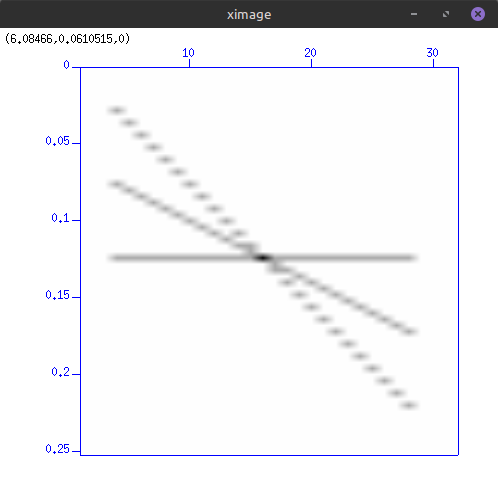
\includegraphics[width=.72\textwidth]{16suplane1.png}
\caption{Exemplo de seção sintética gerada pelo \texttt{suplane}.}
\end{figure}

\subsection{Coordenadas de fonte e receptor}

O comando \texttt{sushw} foi utilizado para preencher as coordenadas
horizontais da fonte e dos receptores:

\begin{lstlisting}[language=bash]
sushw key=sx,gx a=0,400 b=20,20 < dado.su > dado2.su
sugethw key=sx,gx < dado2.su
\end{lstlisting}

Assim, a fonte começa em 0 m, o receptor em 400 m e ambas as posições
avançam 20 m a cada traço. O uso de \texttt{sugethw} permite verificar
diretamente os valores gravados nos cabeçalhos.

\subsection{Estrutura binária do formato SU}

Cada traço SU é descrito como um cabeçalho de 240 bytes seguido das amostras
em ponto flutuante de 32 bits. Para $N$ traços, cada um com $n_s$ amostras,
o tamanho aproximado do arquivo é

\[
  N\left(240 + 4n_s\right)\ \text{bytes}.
\]

No exemplo com 1000 traços e 120 amostras, isso resulta em
$(1000)(240+4\cdot120)=720\,000$ bytes.

\section{Convolução, wavelet Ricker e filtros}

\subsection{Convolução de sinais discretos}

O script \texttt{convolucao.m} verifica numericamente que a convolução
de sinais finitos com $m$ e $n$ amostras possui $m+n-1$ amostras. O exemplo
usa sinais de 10 e 15 amostras e, em seguida, substitui os sinais nulos por
um pulso e um filtro simples para visualizar o resultado.

\begin{figure}[H]
\centering
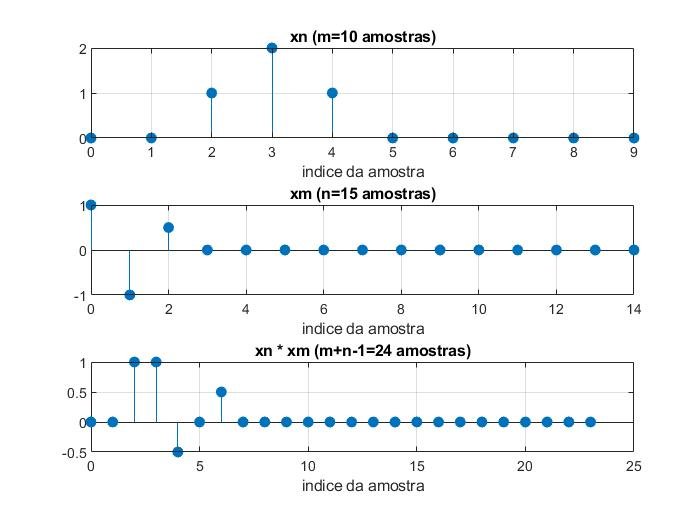
\includegraphics[width=.85\textwidth]{convolucao.jpg}
\caption{Convolução de sinais discretos: sinais de entrada e resultado da convolução.}
\label{fig:convolucao-sinais}
\end{figure}

\subsection{Pulso Ricker}

O arquivo \texttt{gerar\_pulso\_ricker.m} implementa a wavelet Ricker em
uma janela simétrica de $-0{,}1$ a $0{,}1$ s. A frequência de pico é obtida
a partir do primeiro zero temporal $t_0$:

\[
f_p=\frac{1}{\sqrt{2}\,\pi t_0},
\]

e a wavelet é calculada por

\[
w(t)=\left(1-2(\pi f_p t)^2\right)
\exp\left(-(\pi f_p t)^2\right).
\]

\subsection{Operadores de diferenças}

O script \texttt{convolucao2.m} aplica a uma wavelet Ricker de 20 Hz,
amostrada a cada 4 ms, os operadores

\[
p=\frac{1}{2\Delta t}[1,0,-1],
\qquad
q=\frac{1}{\Delta t^2}[1,-2,1].
\]

\begin{figure}[H]
\centering
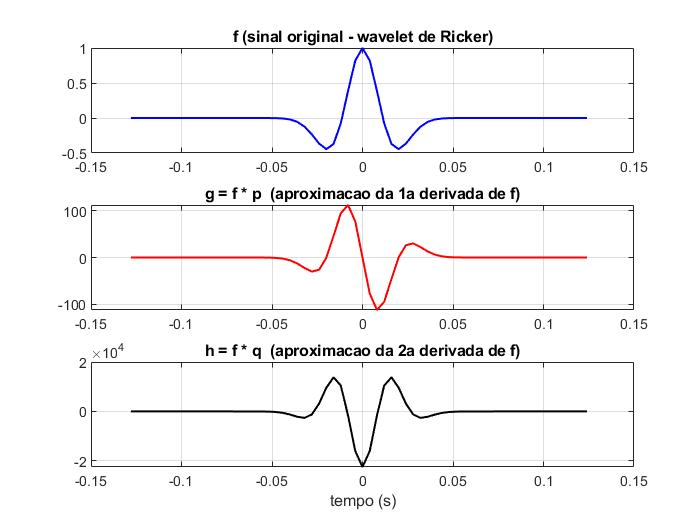
\includegraphics[width=.85\textwidth]{convolucao2.jpg}
\caption{Aplicação dos operadores de diferenças à wavelet Ricker: sinal original, primeira derivada aproximada e segunda derivada aproximada.}
\label{fig:operadores-diferencas}
\end{figure}

As convoluções $g=f*p$ e $h=f*q$ são interpretadas como aproximações,
respectivamente, da primeira e da segunda derivada de $f$. A primeira
derivada destaca transições e cruza zero em extremos locais; a segunda
destaca a curvatura e tende a realçar componentes de alta frequência.



\section{Modelagem 1D por refletividade}

O fluxo principal está implementado em \texttt{questao11.m}. Ele é dividido em três etapas:

\begin{enumerate}
\item definição das profundidades e velocidades das camadas;
\item cálculo dos tempos de ida e volta, coeficientes de reflexão e perdas acumuladas por transmissão;
\item convolução da série de amplitudes com o pulso Ricker e visualização do traço sísmico final.
\end{enumerate}

Para interfaces entre velocidades $v_i$ e $v_{i+1}$, o coeficiente de
reflexão utilizado é

\[
r_i=\frac{v_{i+1}-v_i}{v_{i+1}+v_i}.
\]

O programa exibe o perfil de refletividade, o perfil de amplitudes após as
perdas de transmissão e o traço final convolvido. O intervalo de
amostragem configurado no exemplo é de 2 ms e o primeiro zero do pulso é
$t_0=25$ ms.

\begin{figure}[H]
\centering
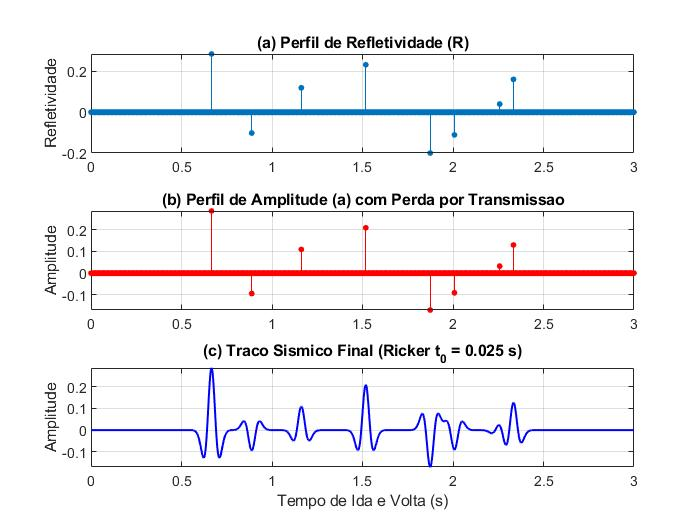
\includegraphics[width=.75\textwidth]{questao11.jpg}
\caption{Traço sísmico obtido da convolução do perfil de refletividade e do perfil de amplitude}
\end{figure}

Ao aumentar a espessura das interfaces, vemos que o tempo de ida e volta no \textit{plot} aumenta, porque a onda vai propagar por uma distância maior.

\begin{figure}[H]
\centering
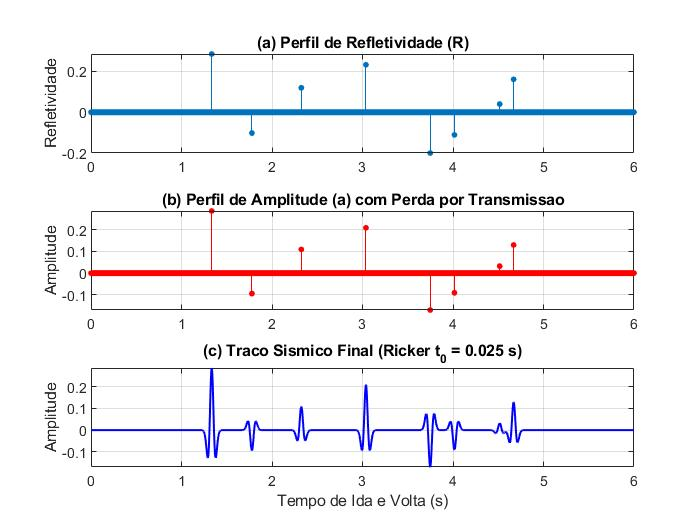
\includegraphics[width=.75\textwidth]{questao11-2z.jpg}
\caption{Traço sísmico obtido da convolução do perfil de refletividade e do perfil de amplitude, com maior distância entre interfaces}
\end{figure}

Ao aumentar as velocidades das interfaces, vemos que o tempo de ida e volta no \textit{plot} diminui.

\begin{figure}[H]
\centering
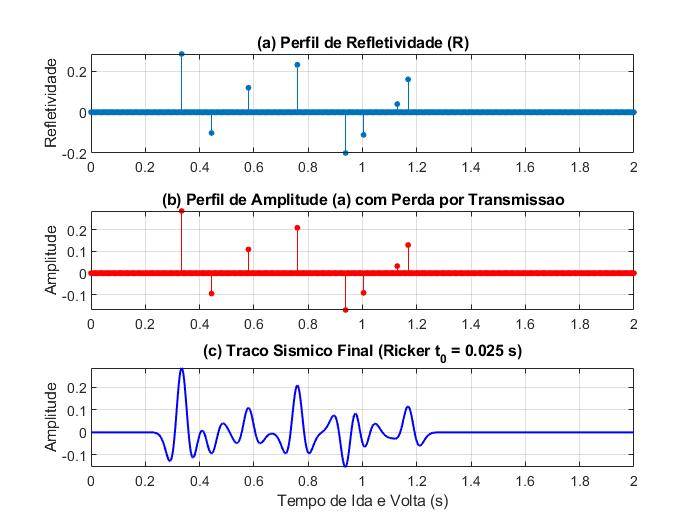
\includegraphics[width=.75\textwidth]{questao11-2v.jpg}
\caption{Traço sísmico obtido da convolução do perfil de refletividade e do perfil de amplitude, com maior velocidades de propagação nas interfaces}
\end{figure}

\section{Modelagem e Aquisição 2D}

\subsection{Aquisição sintética com \texttt{susynlv}}

A geração de dados sintéticos com um refletor plano inclinado foi feita conforme as seguintes especificações:

\begin{itemize}
\item aquisição zero-offset com 101 tiros espaçados de 0,05 km;
\item aquisição common-offset com afastamento de 500 m;
\item validação de \texttt{sx}, \texttt{gx} e \texttt{offset} por
      \texttt{sugethw};
\item seção common-shot com 161 receptores entre $-4$ e $4$ km;
\item visualização em função do número do tiro, da posição e do offset.
\end{itemize}

O resultado dessa aquisição pode ser visualizado na figura a seguir

\begin{figure}[H]
\centering
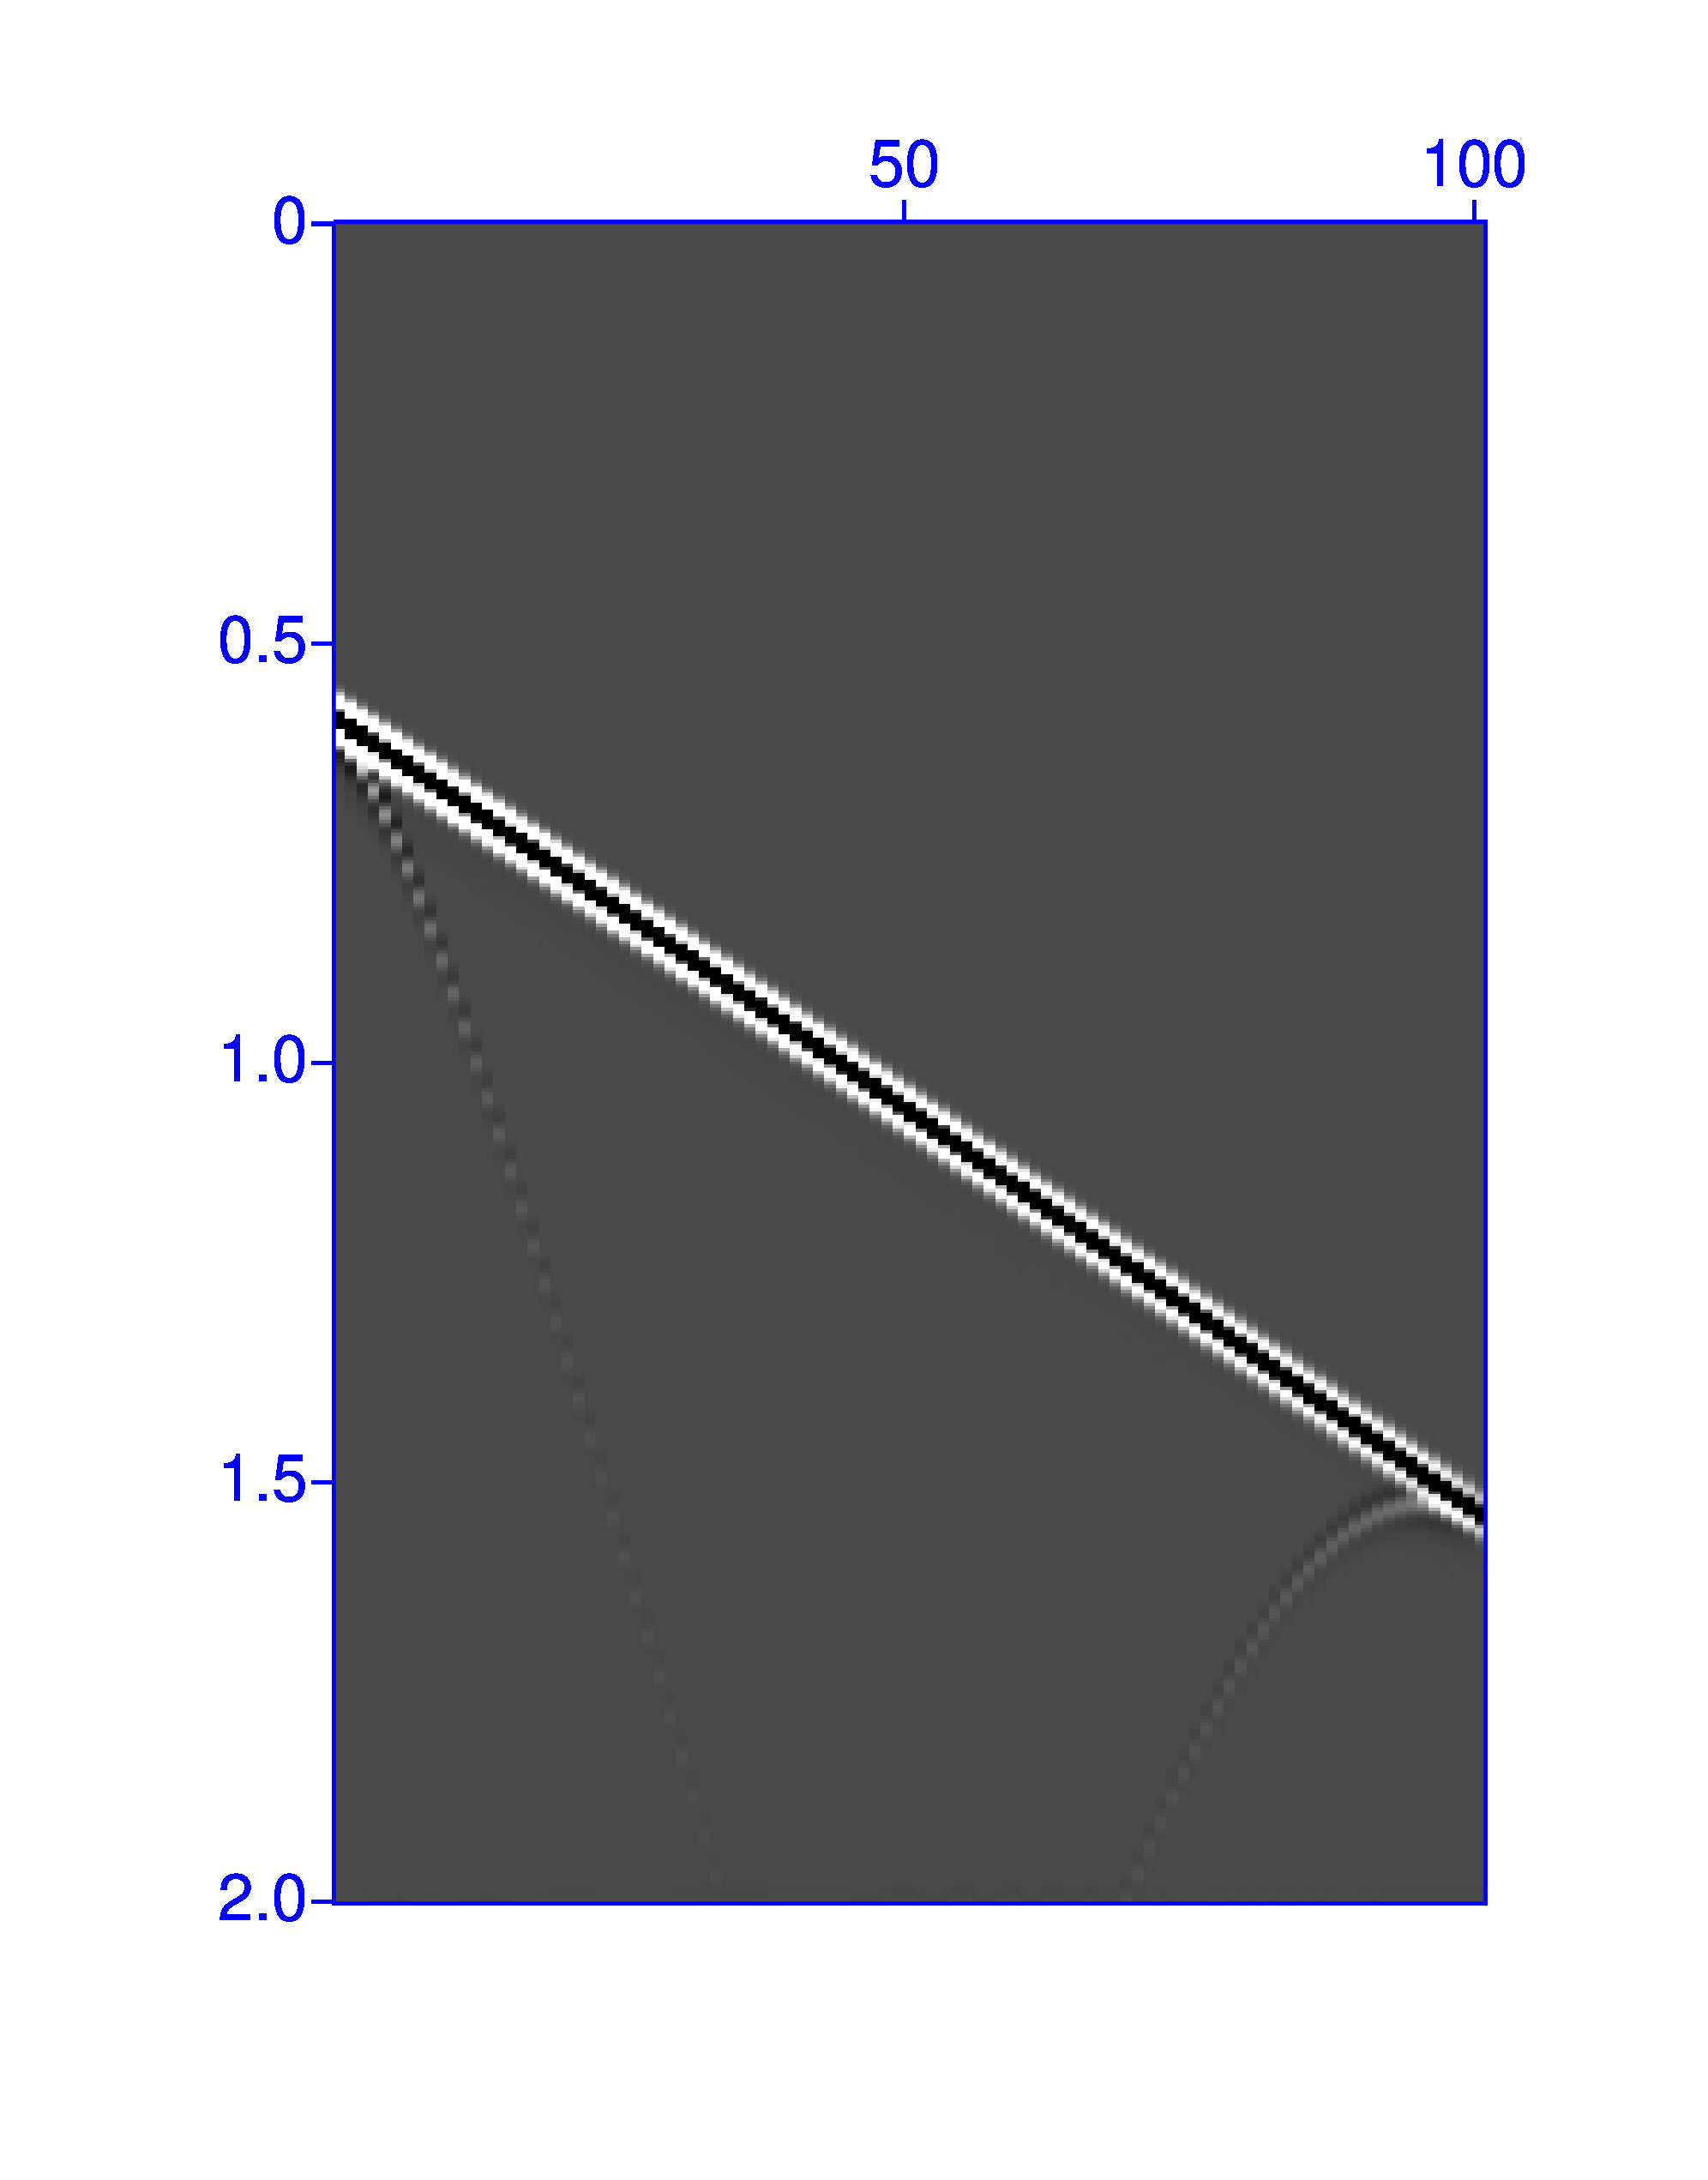
\includegraphics[width=.5\textwidth]{c2-c-tiros-offset-500.jpg}
\caption{Exemplo de aquisição com offset constante de 500 m.}
\end{figure}

\subsection{Modelos de velocidade e diferenças finitas}

\subsection{Modelo estratificado}

O script \texttt{modelo\_velocidades\_2d.m} cria uma malha de 600 pontos em
profundidade por 1600 pontos na horizontal. São atribuídas velocidades de
1500, 2000, 3000 e 4000 m/s a quatro intervalos de profundidade. A matriz
é gravada no arquivo \texttt{vel.out} em formato binário little-endian
\texttt{float32}.

\subsection{Modelo com difratores}

O script \texttt{modelo\_velocidades\_2d\_difratores.m} parte do mesmo
modelo estratificado e adiciona duas pequenas regiões com velocidade de
4000 m/s, representando pontos difratores. O resultado é salvo como
\texttt{vel-difrator.out}.

\begin{figure}[H]
\centering
\begin{minipage}{.47\textwidth}
\centering
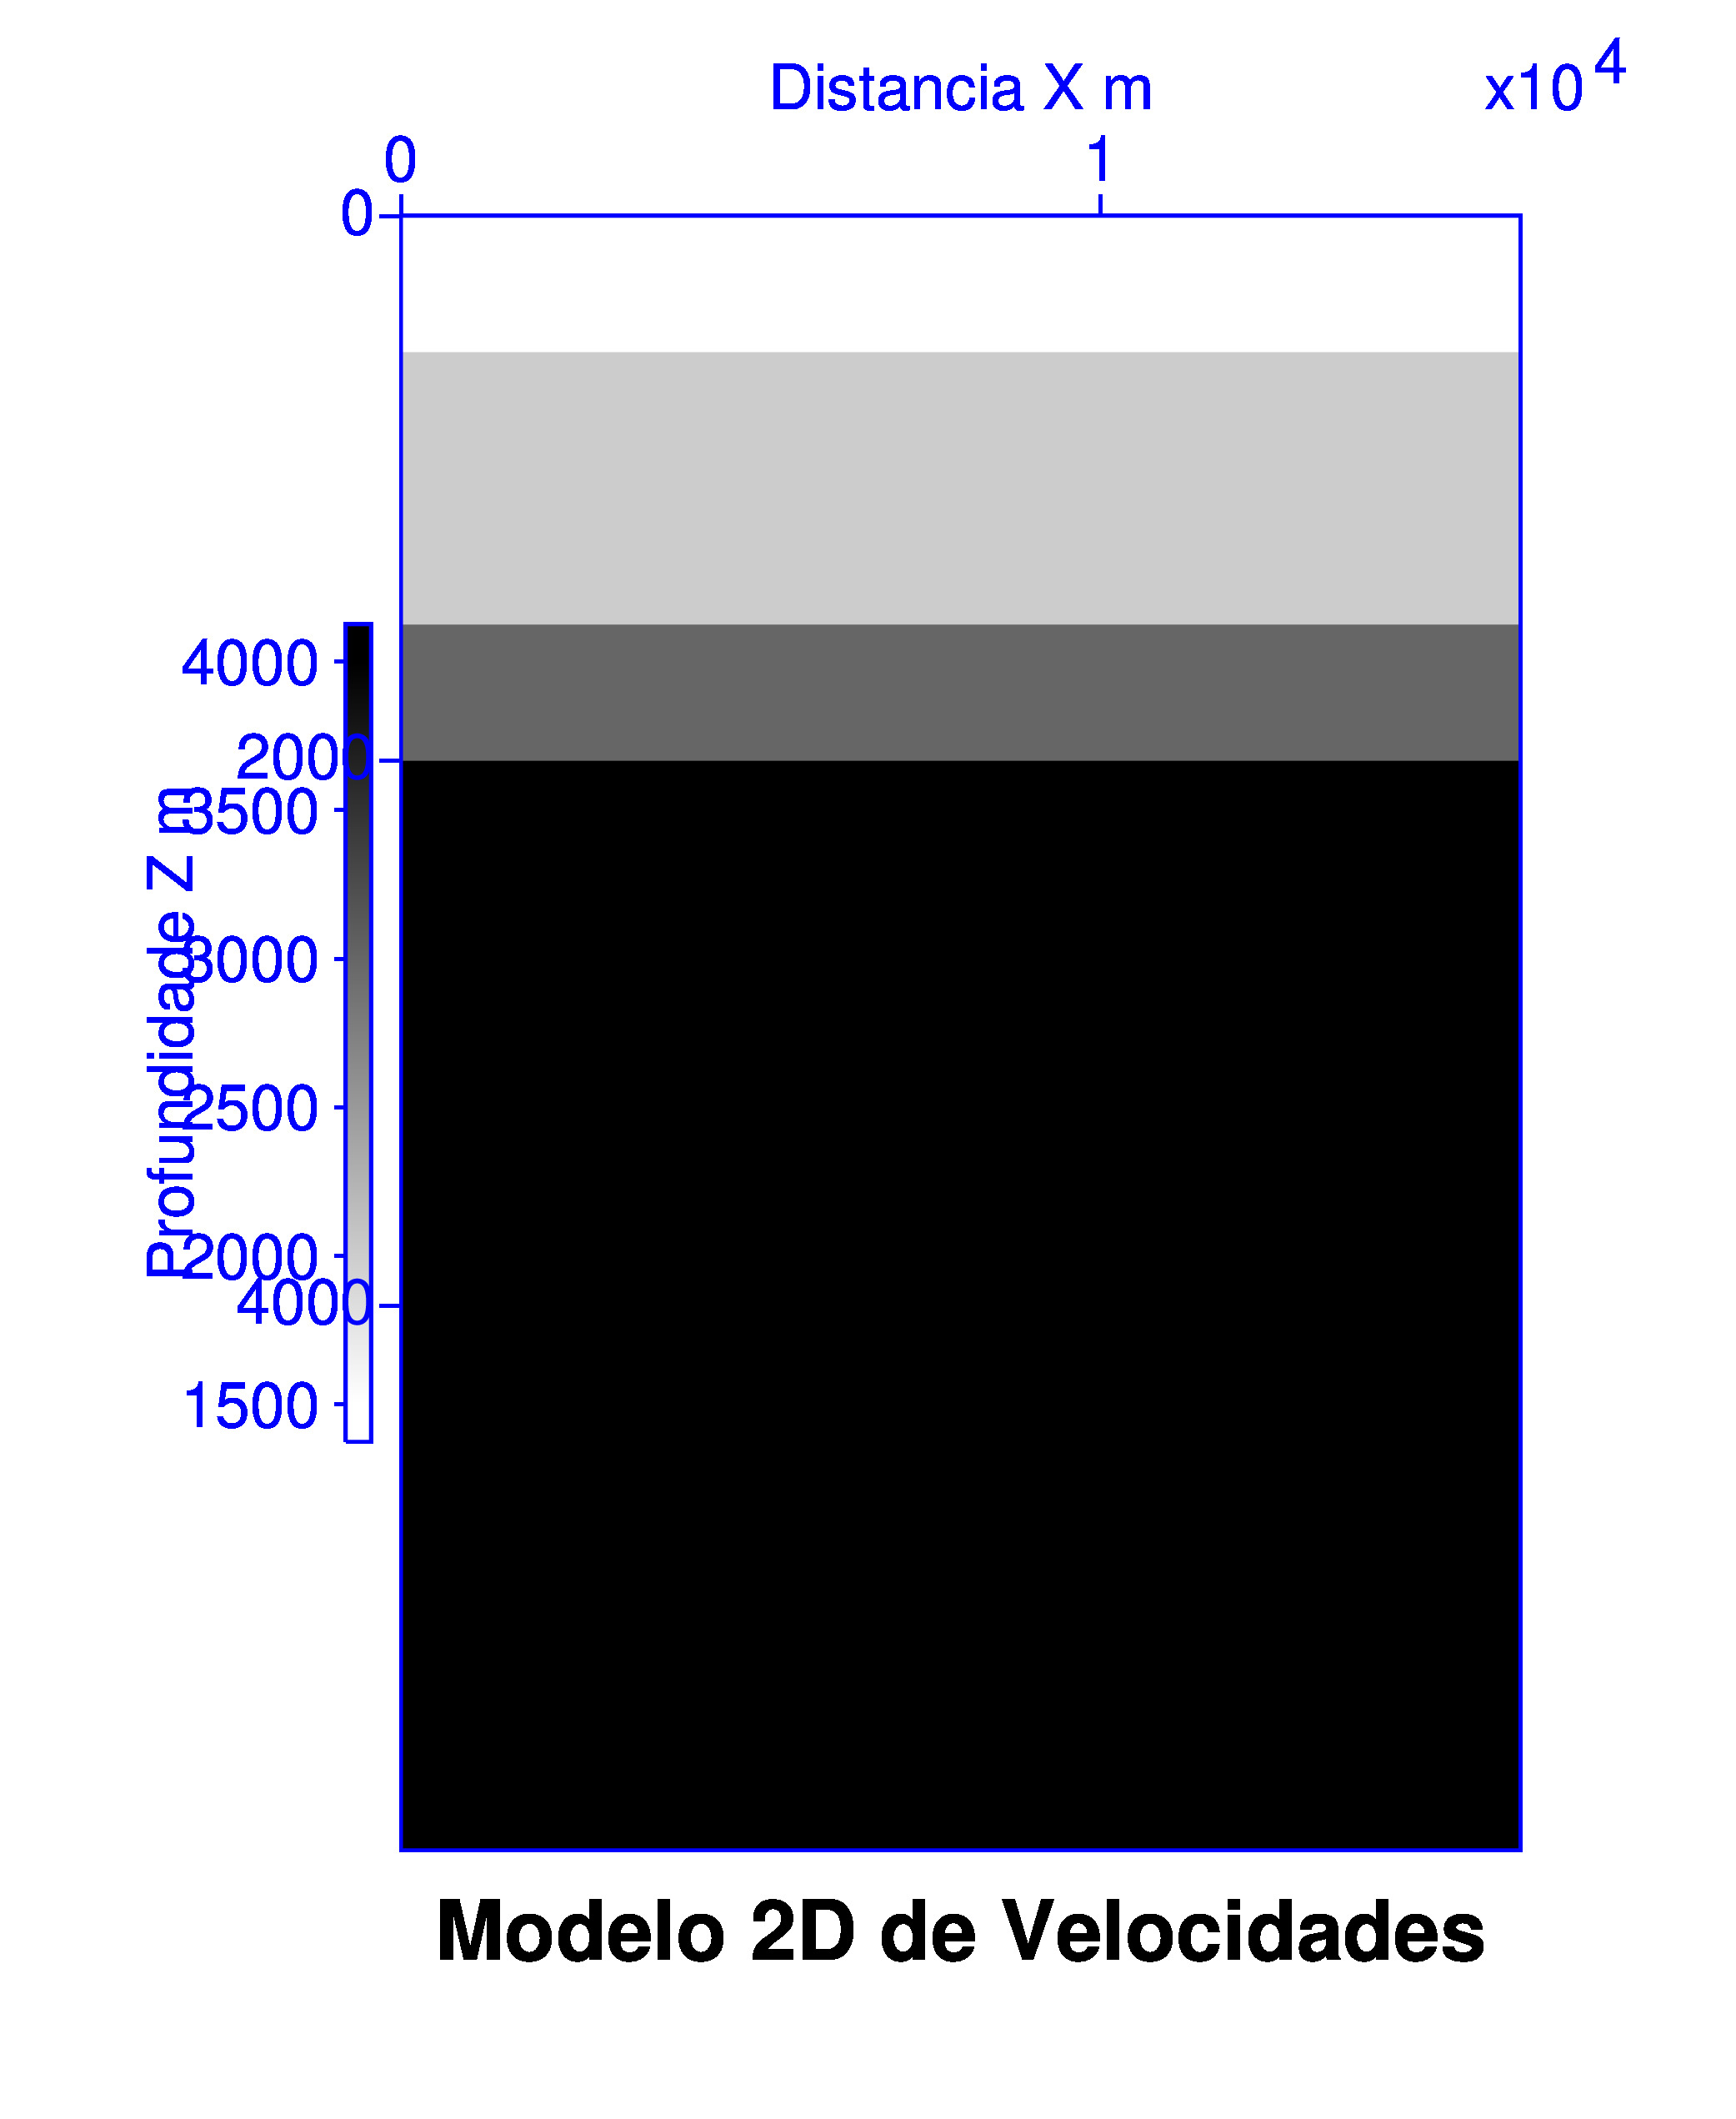
\includegraphics[width=\textwidth]{velocidades.jpg}
\captionof{figure}{Modelo estratificado.}
\end{minipage}
\hfill
\begin{minipage}{.47\textwidth}
\centering
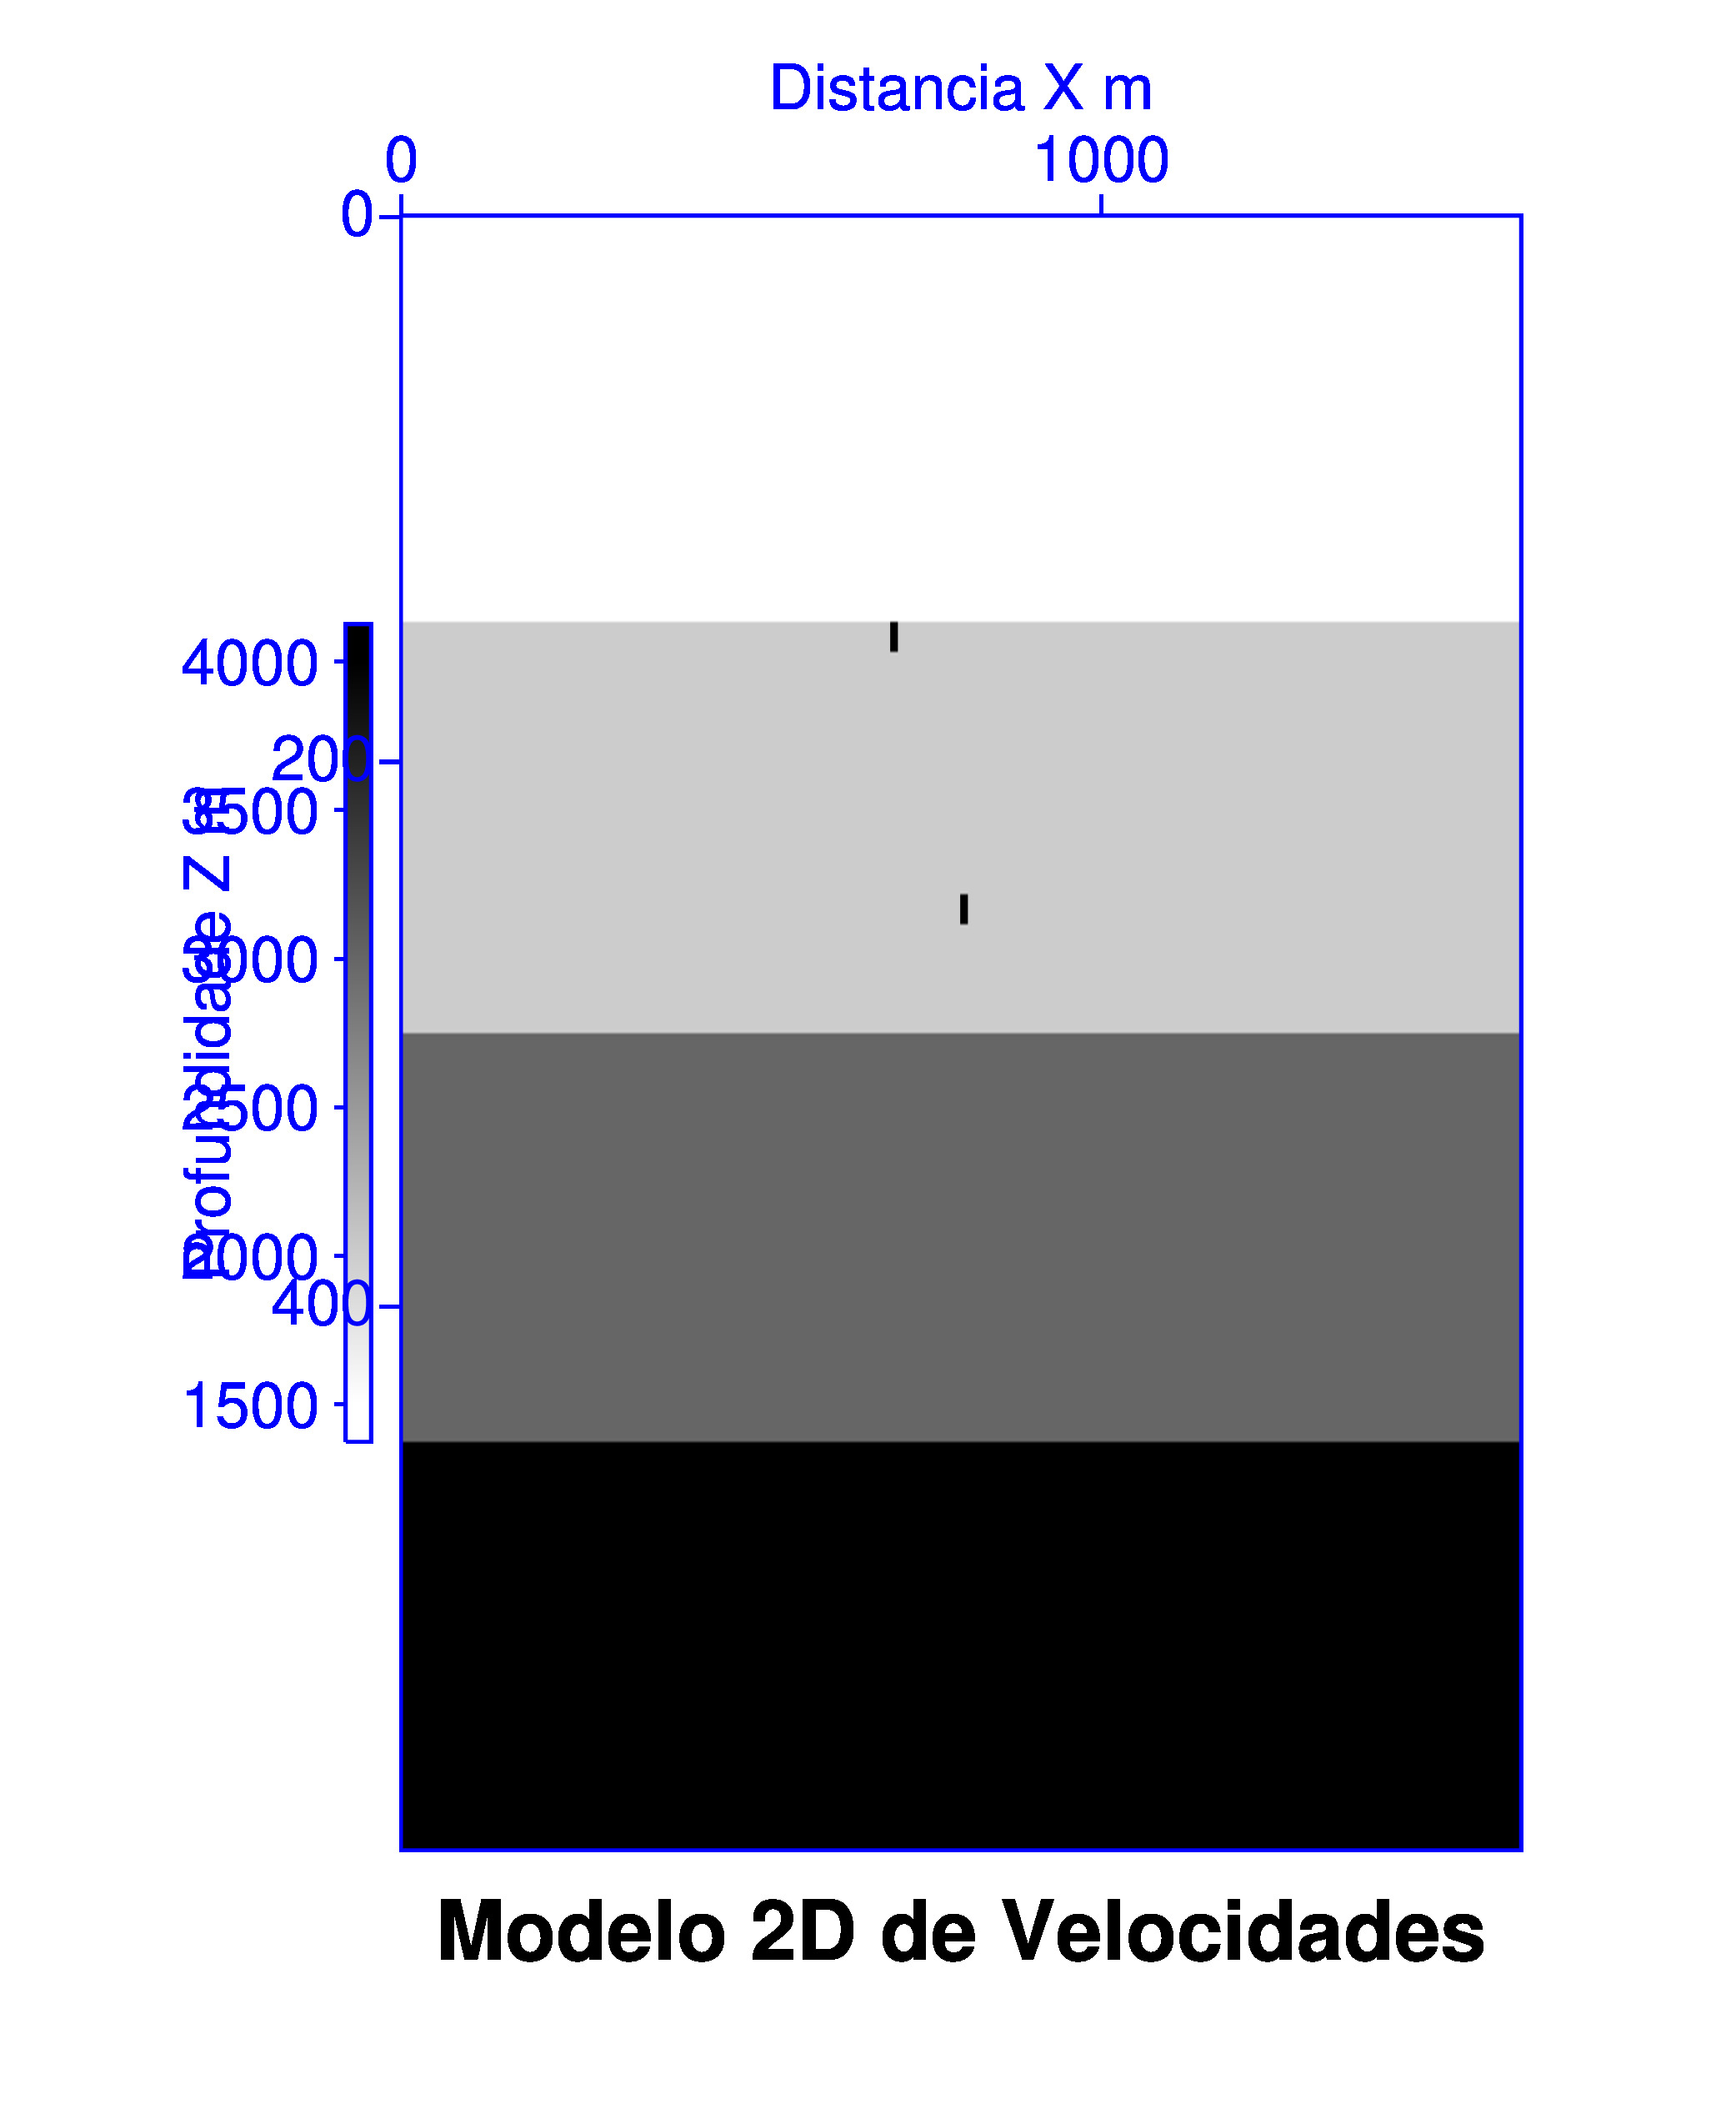
\includegraphics[width=\textwidth]{velocidades-difratores.jpg}
\captionof{figure}{Modelo com difratores.}
\end{minipage}
\end{figure}

\subsection{Simulação da aquisição}

Os scripts \texttt{simular-aquisicao.sh} e
\texttt{simular-aquisicao-tiros.sh} automatizam chamadas ao
\texttt{sufdmod2\_pml}. O primeiro simula um tiro com fonte no centro da
superfície; o segundo percorre a linha com dez posições de fonte, avançando
200 m entre tiros. Em ambos os fluxos, os cabeçalhos dos traços são
ajustados com

\begin{lstlisting}[language=bash]
suchw < hseis.pml.out key1=gx key2=sx key3=offset b=1 c=1
\end{lstlisting}

Essa operação pode ser interpretada como a manipulação da relação
\[
\text{gx} = \text{sx} + \text{offset},
\]
que é equivalente à expressão
\[
\text{offset} = \text{gx} - \text{sx}.
\]
Assim, conhecendo a posição da fonte e o afastamento, calcula-se a posição
do receptor; inversamente, as posições do receptor e da fonte determinam o
offset do traço.

Os arquivos intermediários de onda são removidos ao fim de cada execução,
e os resultados são reunidos em arquivos SU para visualização.

\begin{figure}[H]
\centering
\begin{minipage}{.47\textwidth}
\centering
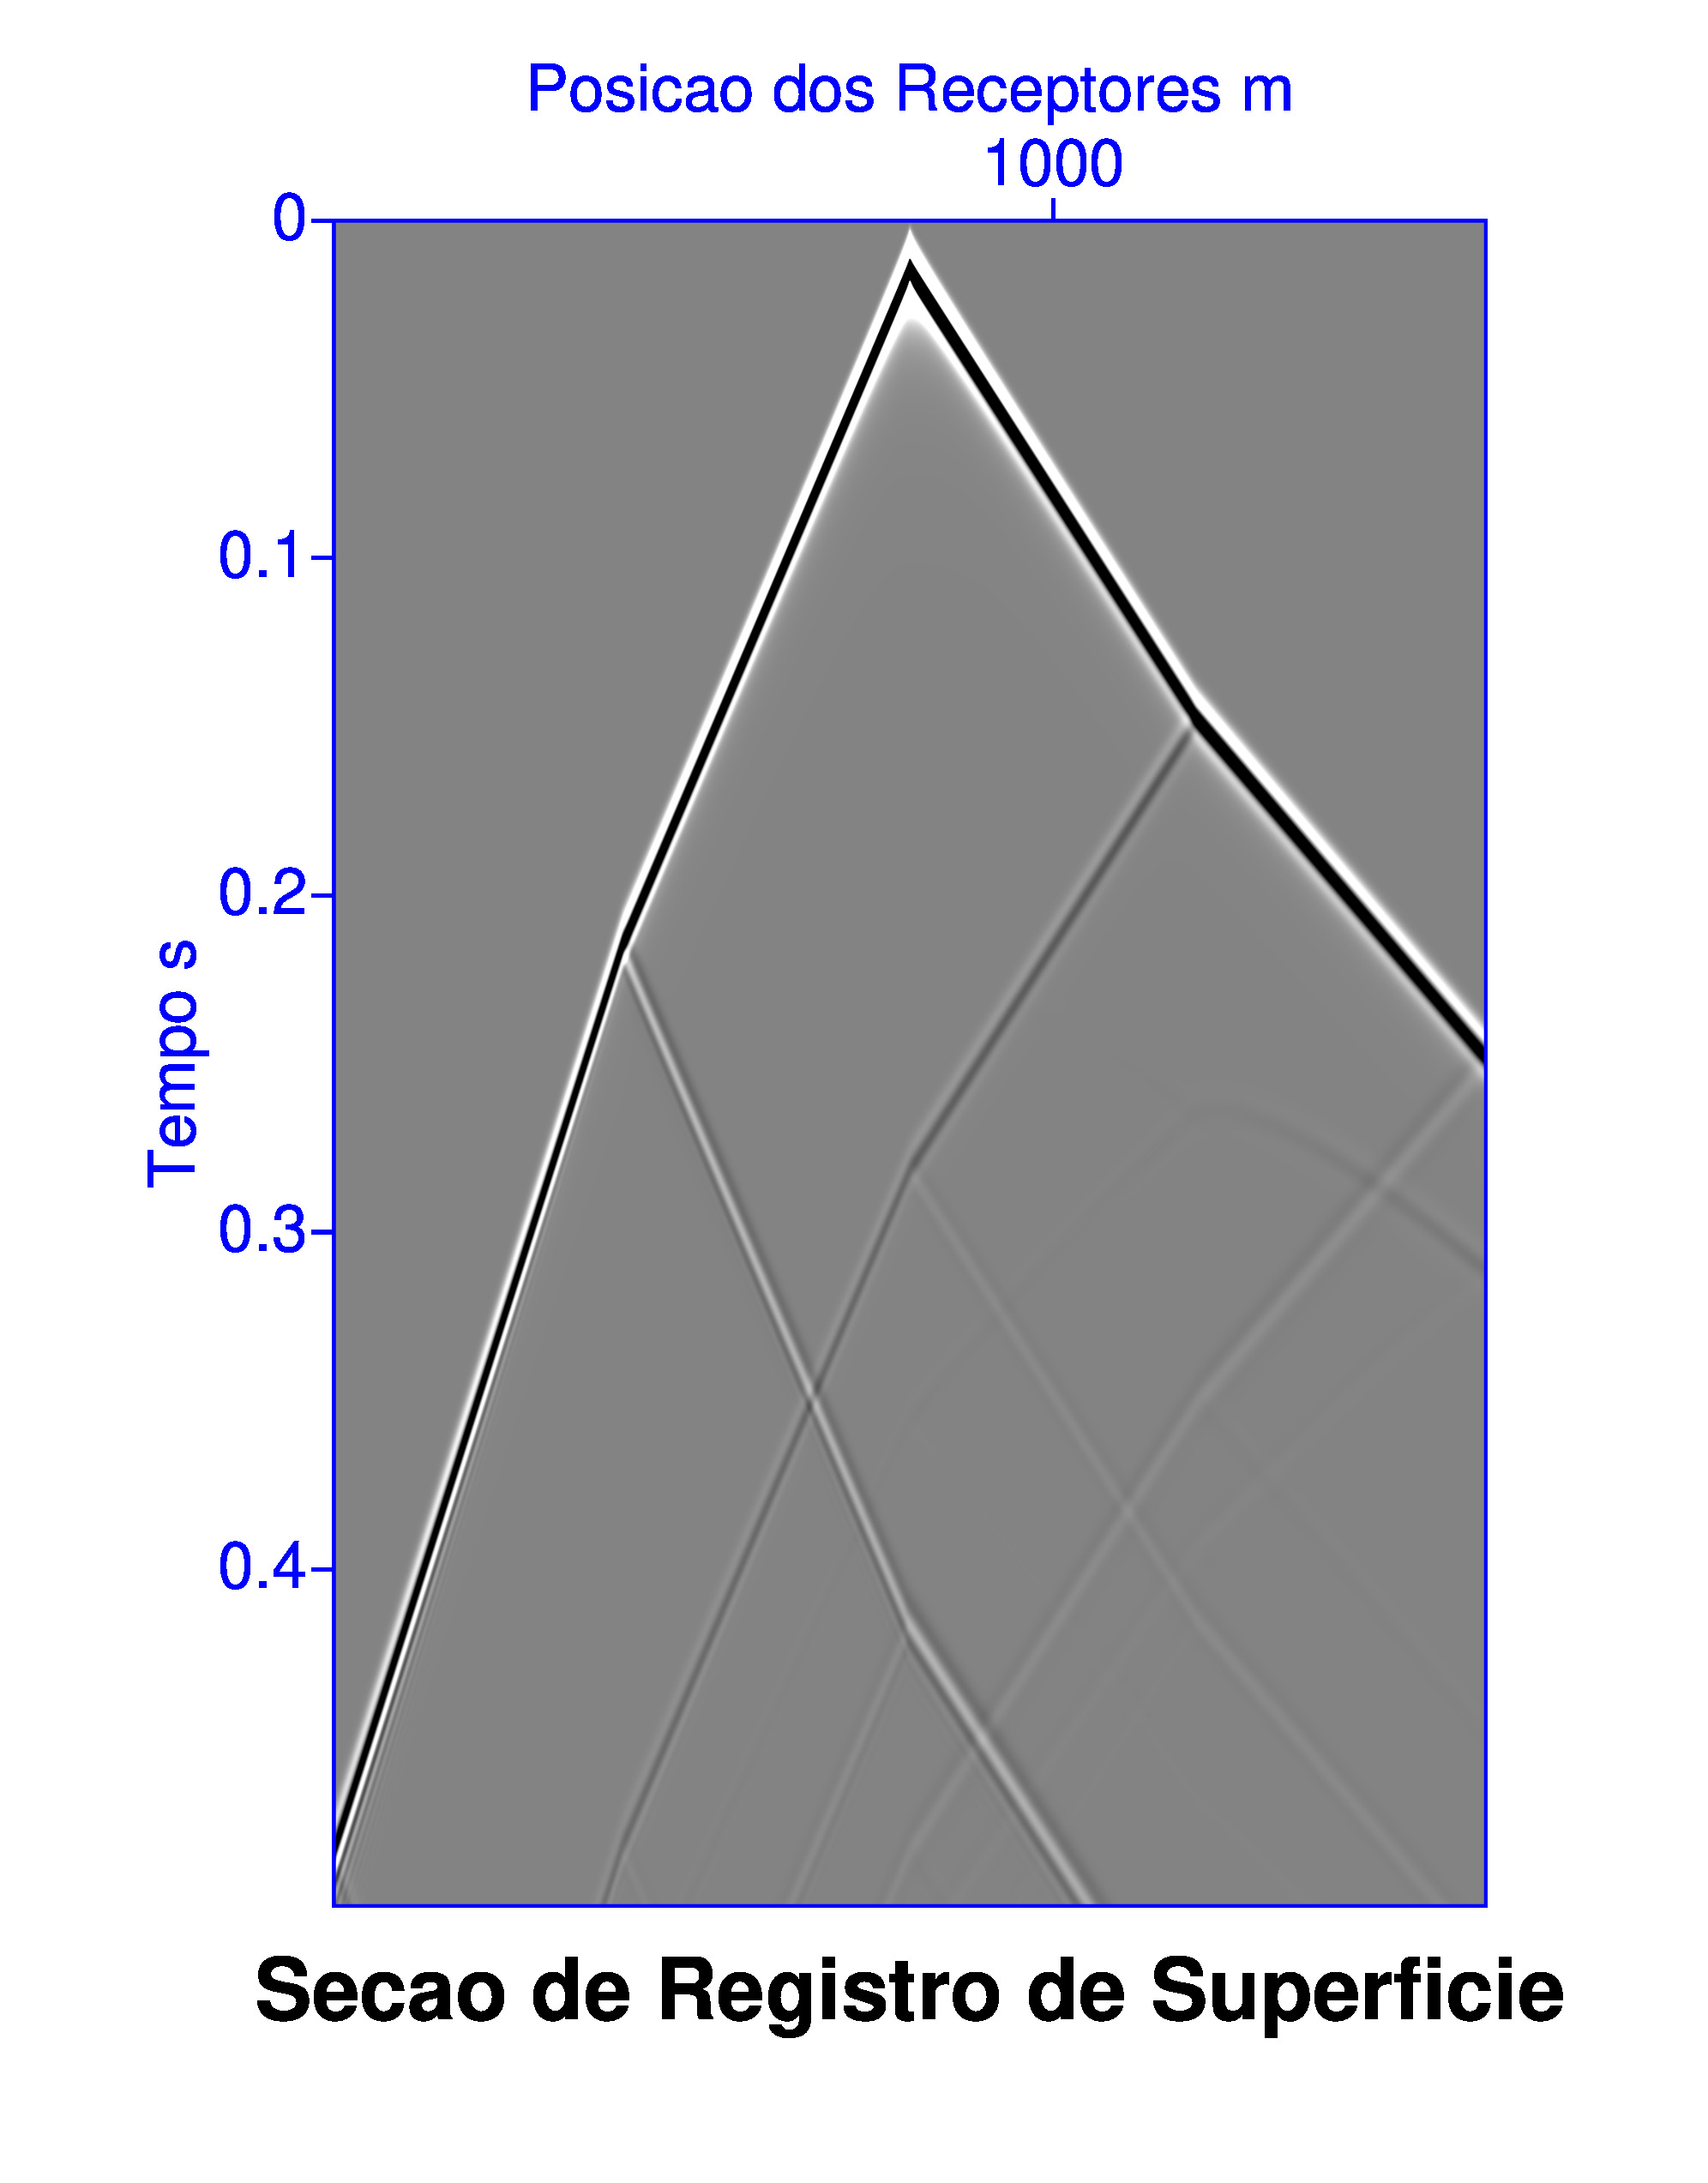
\includegraphics[width=\textwidth]{registro-superficie.jpg}
\captionof{figure}{Registro de superfície simulado para um tiro.}
\end{minipage}
\hfill
\begin{minipage}{.47\textwidth}
\centering
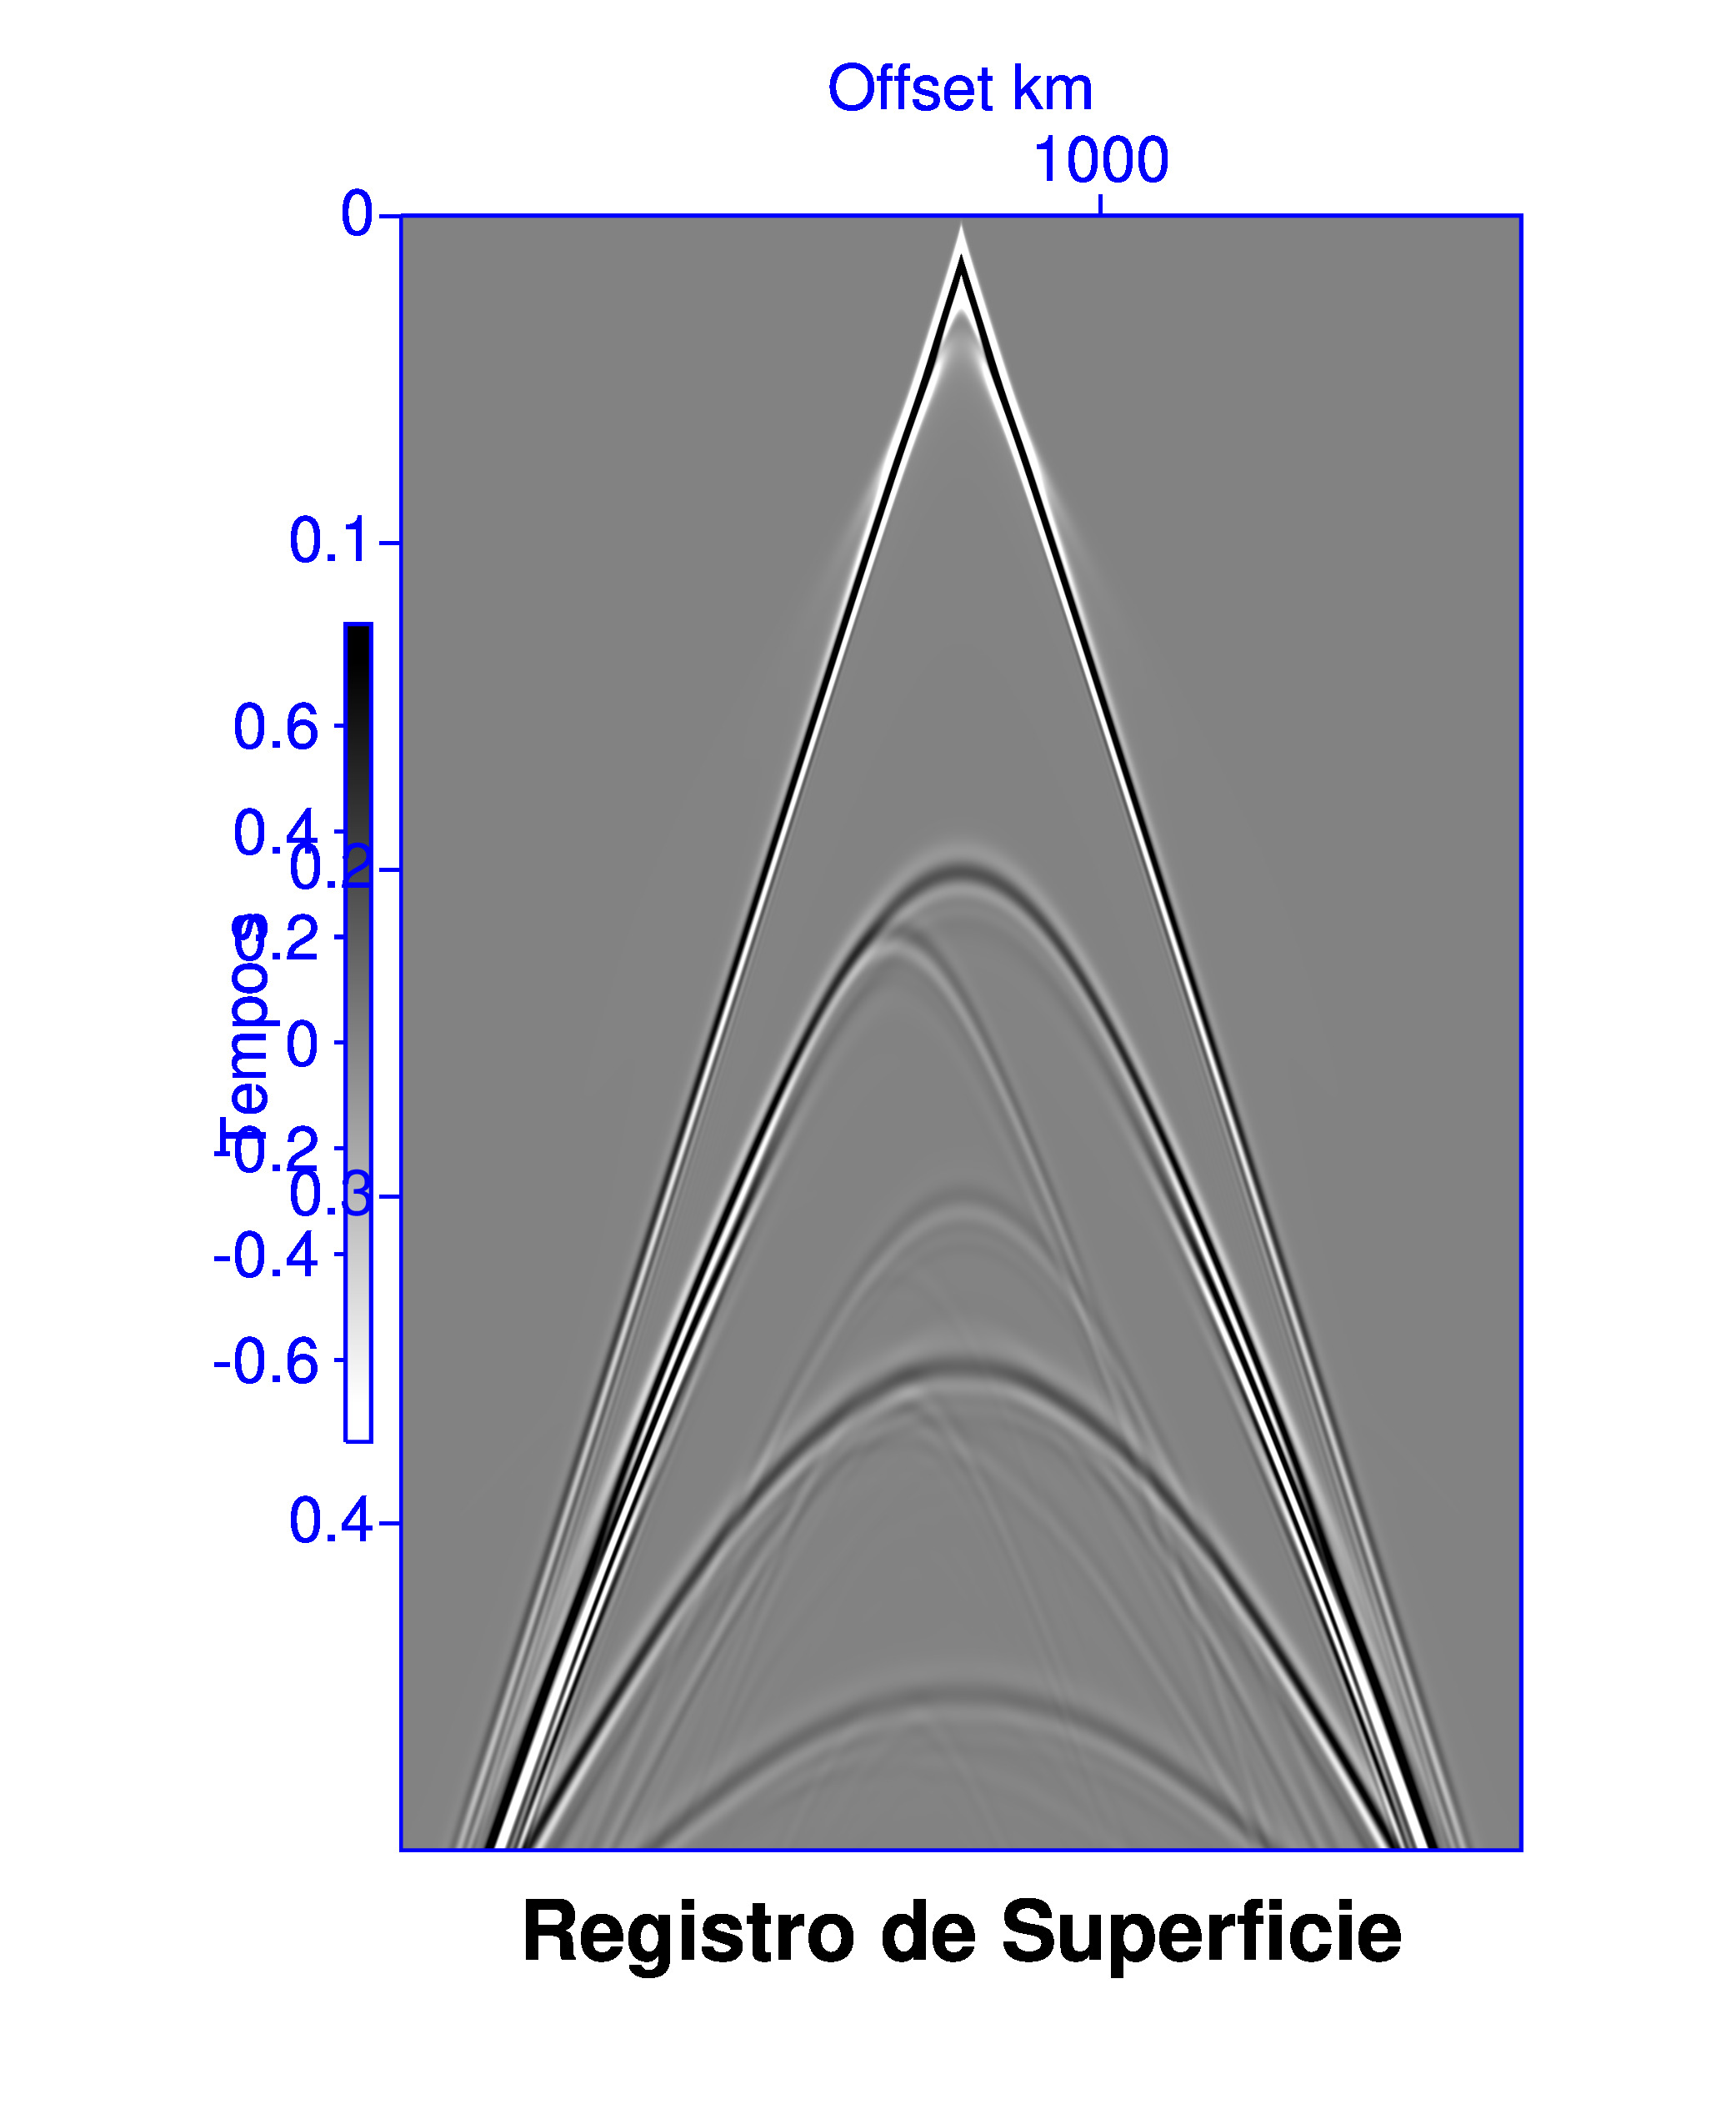
\includegraphics[width=\textwidth]{registro-superficie-difratores.jpg}
\captionof{figure}{Registro de superfície simulado para um tiro com difratores.}
\end{minipage}
\end{figure}

\begin{figure}[H]
\centering
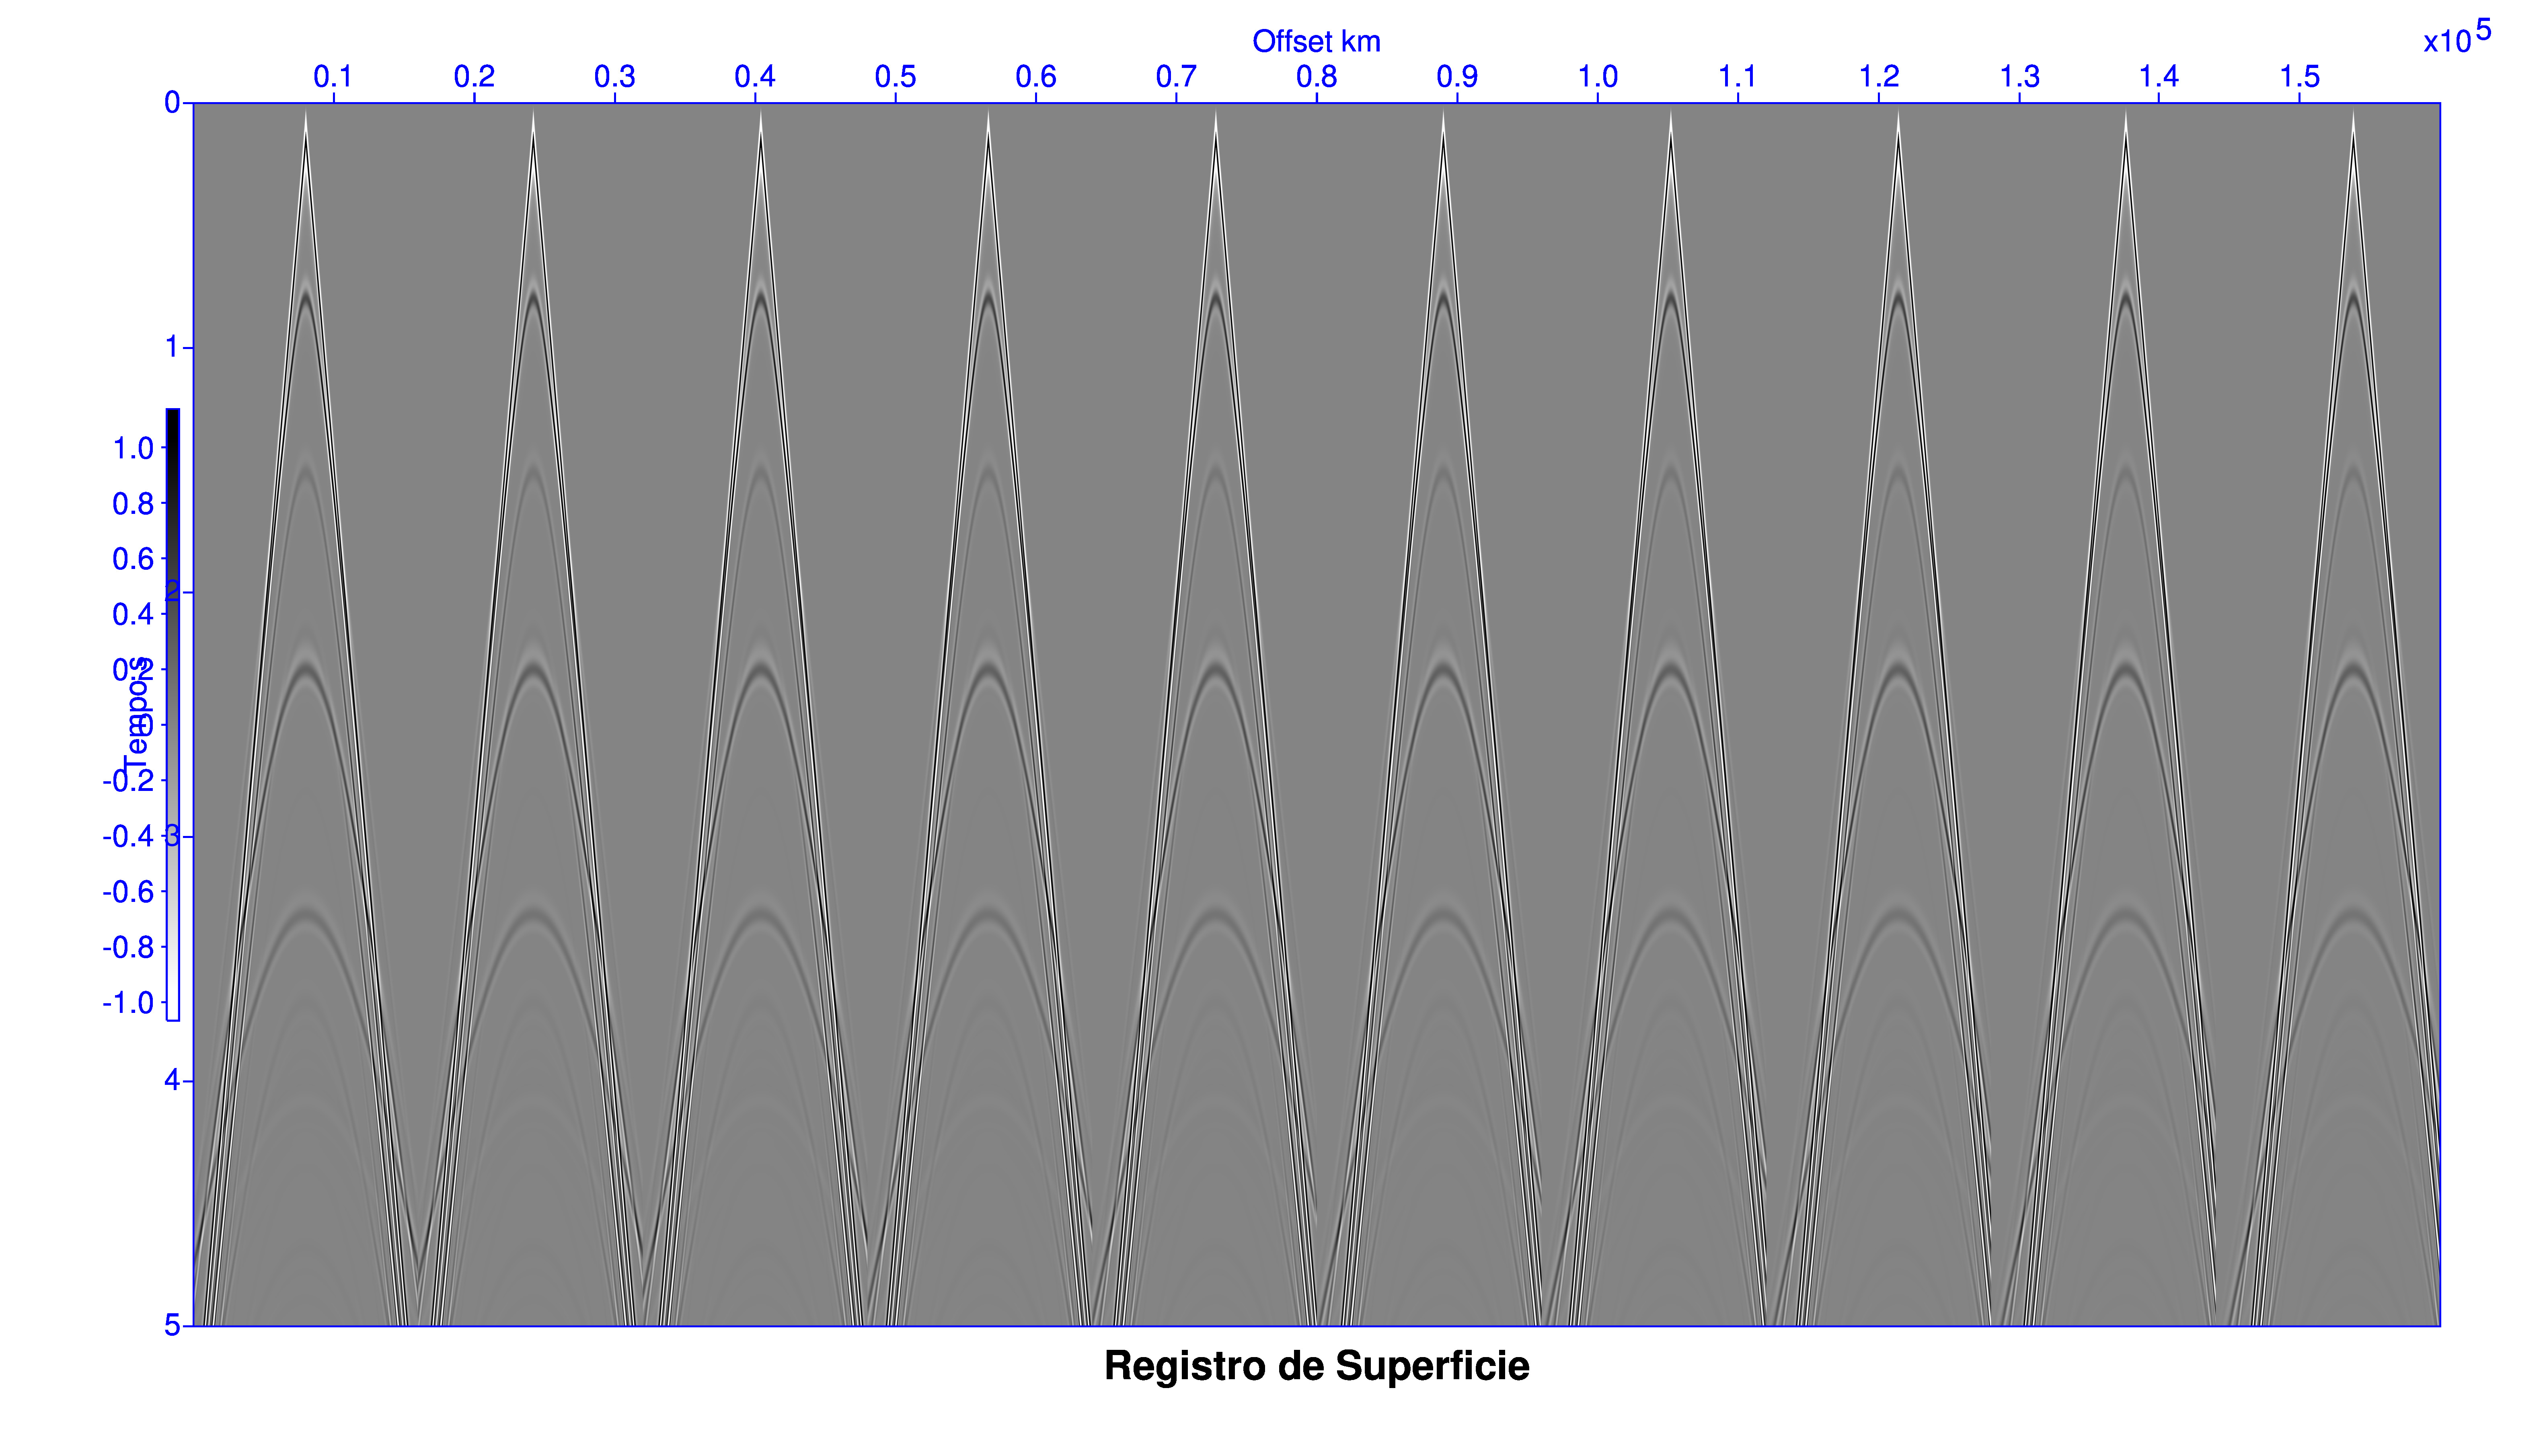
\includegraphics[width=.9\textwidth]{todos_os_tiros.jpg}
\caption{Registro de superfície com múltiplos tiros.}
\end{figure}



\subsection{Organização por CDP}

O script \texttt{calcular-cdp.sh} demonstra o cálculo do ponto de
profundidade comum (CDP) a partir das coordenadas de fonte e receptor:

\begin{lstlisting}[language=bash]
suchw < todos_os_tiros.su key1=cdp key2=gx key3=sx b=0.5 c=0.5
susort cdp offset
\end{lstlisting}

Depois do cálculo, os traços são ordenados por CDP e podem ser visualizados
como uma coleção de gathers. Essa organização é uma etapa importante para
análises posteriores de afastamento comum e empilhamento. Observe que as ondas diretas não foram filtradas. 

Abaixo o plot de todos os traços ordenados por CDP e \textit{offset}

\begin{figure}[H]
\centering
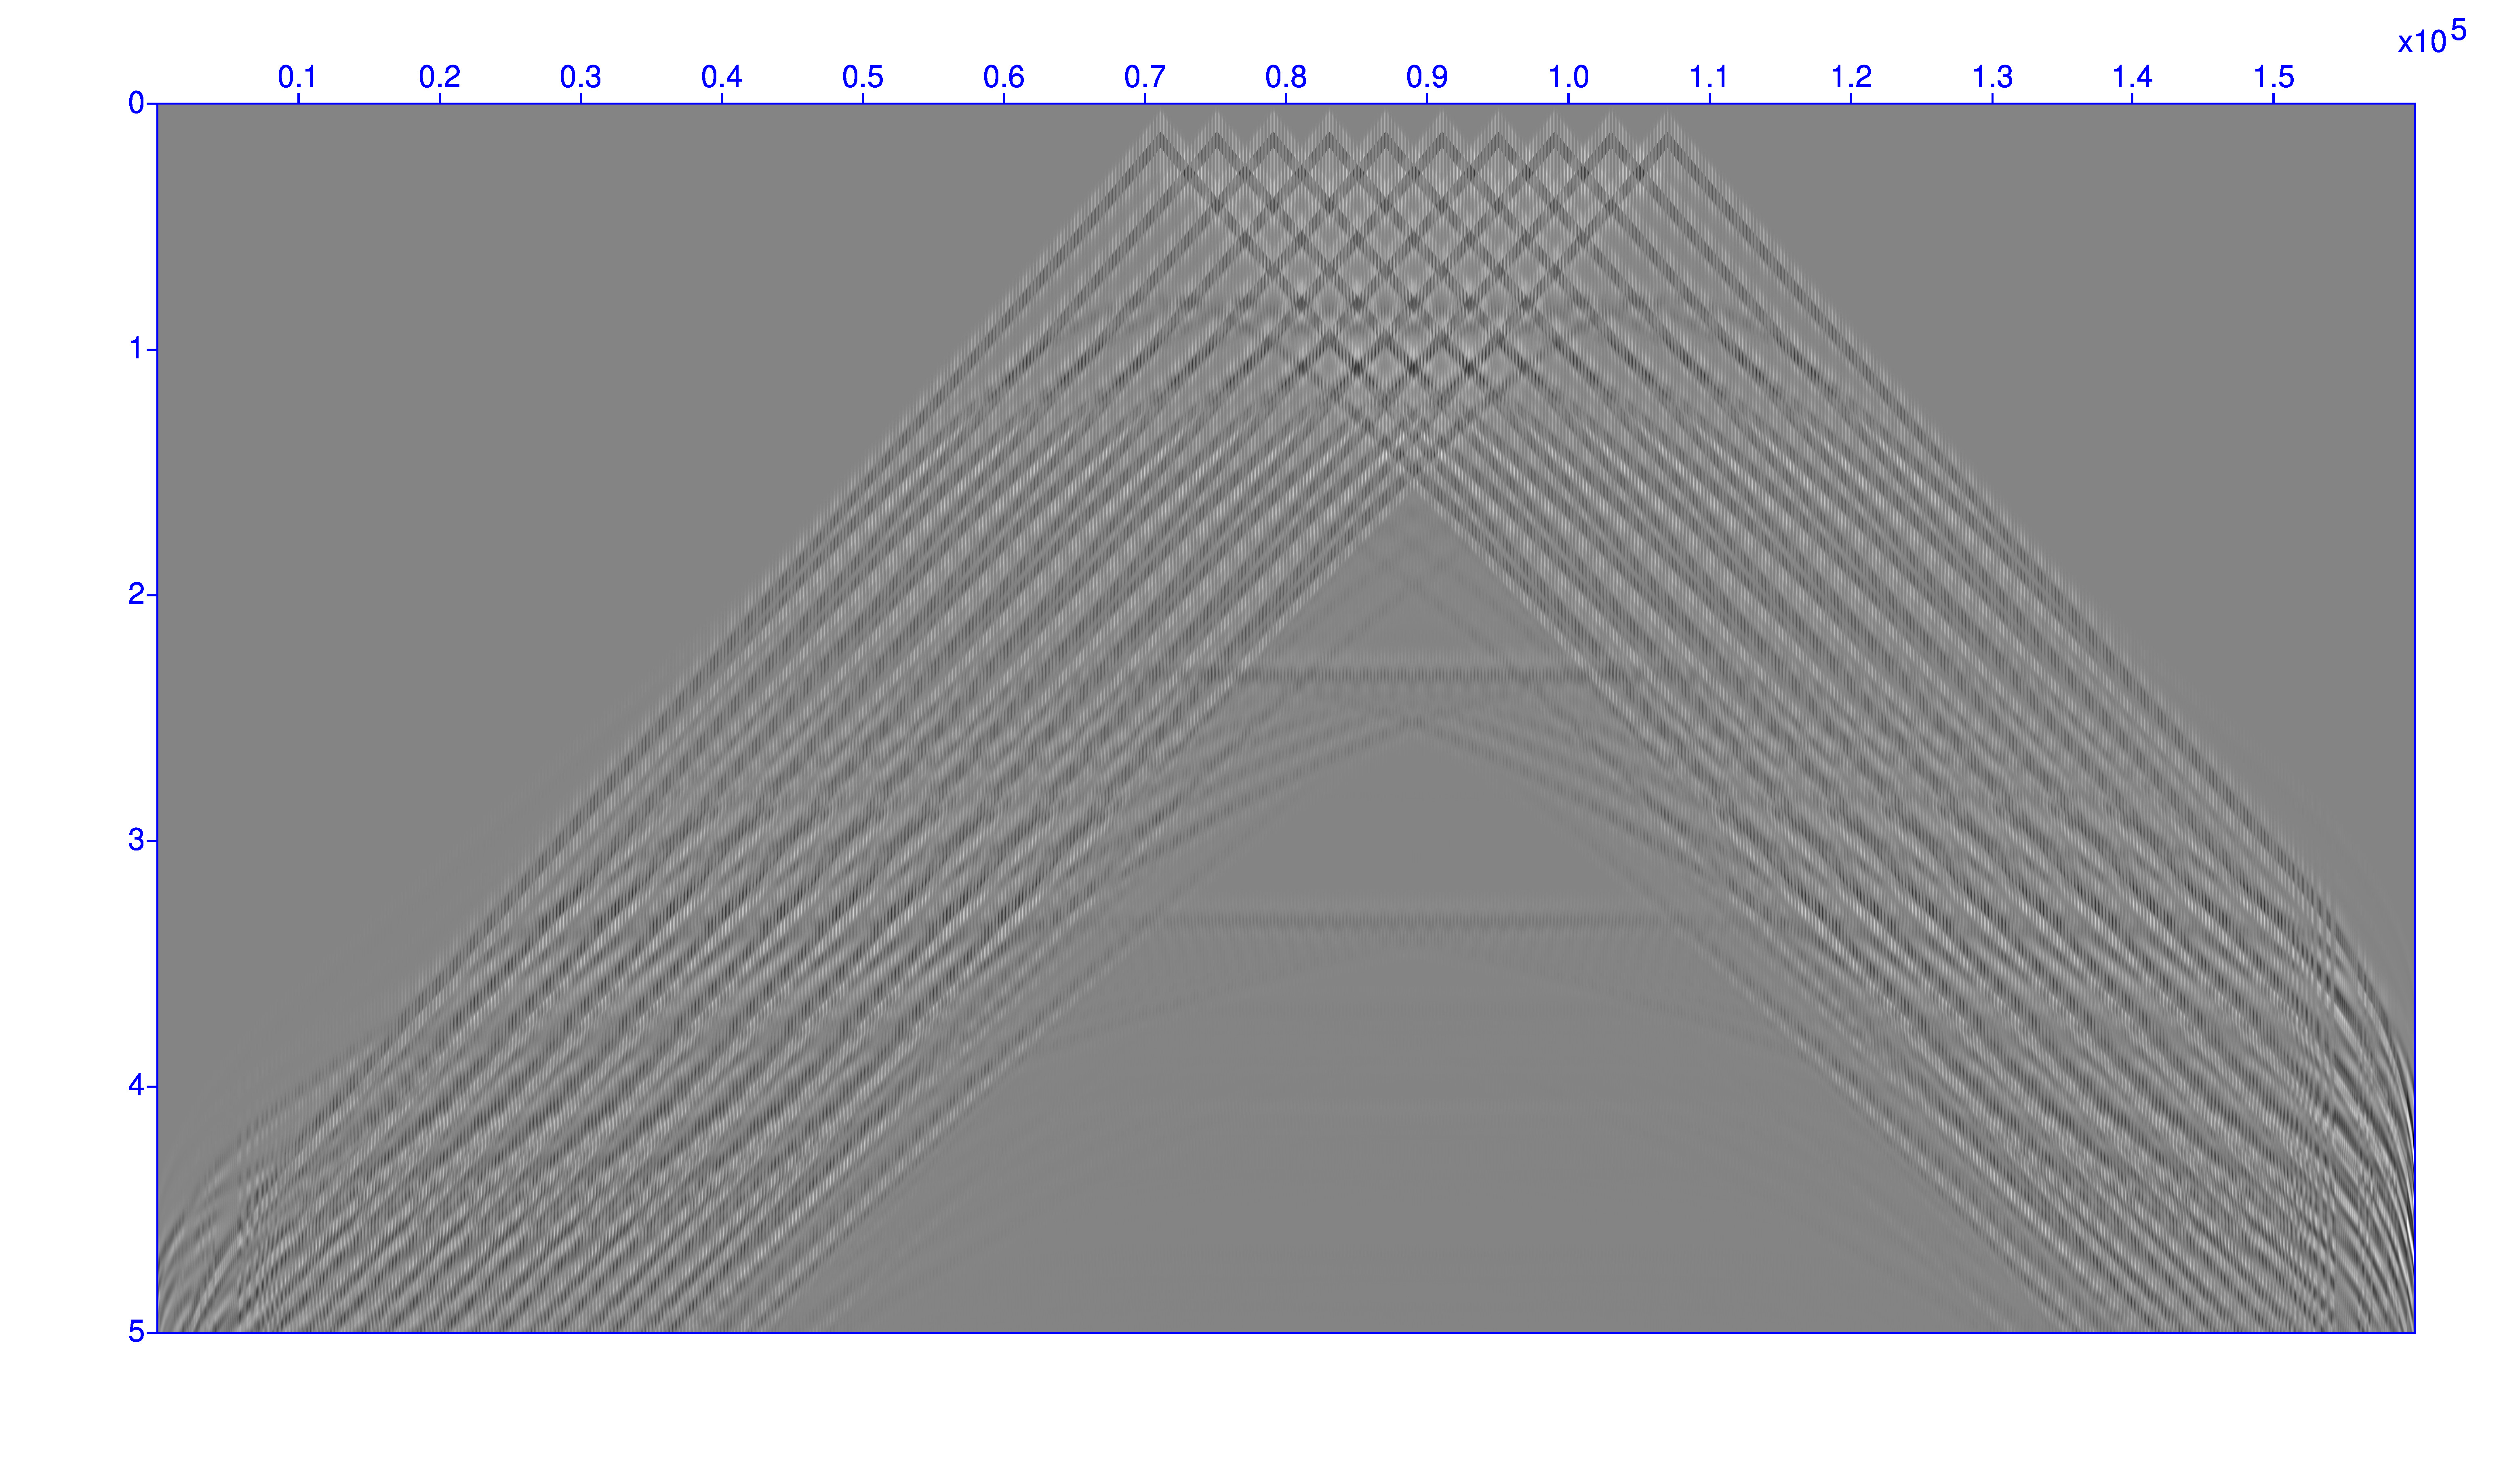
\includegraphics[width=.9\textwidth]{todos_os_tiros_offset_cdp_sorted.jpg}
\caption{Todos os tiros ordenados por CDP e \textit{offset}. No eixo vertical está o tempo de propagação (em segundos) e no horizontal os \textit{offsets} (km)}
\end{figure}


\end{document}